\documentclass{beamer}
\usepackage[T1]{fontenc}

%\documentclass[aspectratio=169]{beamer}
%\usetheme{Madrid} % My favorite!
%\usetheme{Boadilla} % Pretty neat, soft color.
%\usetheme{default}
%\usetheme{Warsaw}
%\usetheme{Bergen} % This template has nagivation on the left
\usetheme{Frankfurt} % Similar to the default 
%with an extra region at the top.
\usecolortheme{seahorse} % Simple and clean template
%\usetheme{Darmstadt} % not so good
% Uncomment the following line if you want %
% page numbers and using Warsaw theme%
% \setbeamertemplate{footline}[page number]
%\setbeamercovered{transparent}
\setbeamercovered{invisible}
\setbeamersize{text margin right=3.5mm, text margin left=7.5mm}  % text margin
% To remove the navigation symbols from 
% the bottom of slides%
%
\usepackage{graphicx}
\usepackage[backend=biber]{biblatex}

\addbibresource{bagneux-14.bib}
\usepackage{tikz}
\usepackage{calc}
\def\checkmark{\tikz\fill[scale=0.4](0,.35) -- (.25,0) -- (1,.7) -- (.25,.15) -- cycle;} 
\def\scalecheck{\resizebox{\widthof{\checkmark}*\ratio{\widthof{x}}{\widthof{\normalsize x}}}{!}{\checkmark}}
%that's defined it - now for a test

\DeclareGraphicsExtensions{.pdf,.png,.jpg}
%\usepackage{bm}         % For typesetting bold math (not \mathbold)
%\logo{\includegraphics[height=0.6cm]{yourlogo.eps}}
%
\title[Trust in Collaborative Marine Networks]{An Investigation into Trust and Reputation Frameworks for Collaborative Teams of Autonomous Underwater Vehicles}

\author{Andrew Bolster}
\institute[UoL]
{
University of Liverpool \\
\medskip
{\emph{andrew.bolster@liv.ac.uk}}\\
\vspace{0.3in}

\includegraphics[width=0.5\textwidth]{img/livuni}%
}
\date{July 3, 2014}
% \today will show current date. 
% Alternatively, you can specify a date.
%
\begin{document}
%

%\AtBeginSection[
%{
%\begin{frame}<beamer>{Table of Contents}
%  \tableofcontents[currentsection,currentsubsection, 
%  hideothersubsections, 
%  sectionstyle=show/shaded,
%  ]
%\end{frame}
%}]
\begin{frame}
  \titlepage
\end{frame}

\frame{\tableofcontents}
\section{Technical Programme}
\subsection{Background and Objectives}
\frame{
\frametitle{Research Context}
\begin{itemize}
  \item Project launched at QUB ECIT in 2011 under the DSTL/DGA Anglo French Defence Research Group PhD Programme 
  \item What lessons from the Mobile Ad Hoc Network (MANET) space can be transferred to the marine environment?
  \item Teams of 3 - 16 Autonomous Underwater Vehicles (AUVs) Mine countermeasures, Hydrography, and Patrol Capabilities (MHPC)
  \item Defence focus, assumption of highly capable enemy attempting to compromise communications / operations
  \item Primary Simulation/Analysis work done in 12/13
  \item Moved to UoL Oct 13 after 2 mth placement @ DSTL PDW Naval Systems / Information Systems departments.
\end{itemize}
}

\frame{
\frametitle{Trust in Ad-Hoc Systems and the context of this document}
\begin{itemize}
  \item Particularly interested in the application of Trust in Decentralised (P2P) Autonomous Systems of Systems, AUVs for example
  \item Trust:\emph{The expectation of an actor performing a certain task or range of tasks within a certain confidence or probability}
  \item Full System Views of Trust
    \begin{itemize}
        \footnotesize
      \item{Design Trust - a system of systems will perform as designed}
      \item\emph{Operational Trust - an individual system will perform as designed in field}
        
  \end{itemize}
  \item Communications not the only target for an attacker (or failure);
    \begin{itemize}
        \footnotesize
        \item Following to restricted area
        \item Masquerading
        \item Hardware Degradation
        \item Resource attack via propulsive power
    \end{itemize}
  \item Physical observation as opportunity to reduce the threat surface while discriminating between 'True' attacks and mechanical failure.
  \item Also could provide additional 'handshake' protocols for 'friendly' fleets/teams through reactionary behaviours
\end{itemize}

}
\subsection{Progress}
\frame{
\frametitle{Multi-Vector Trust and the Threat Surface}
Potential attacks exist across a multi-domain threat surface
\begin{center}
  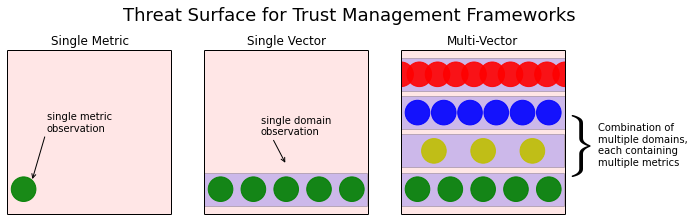
\includegraphics[width=0.9\paperwidth]{img/threat_surface_sum}
\end{center}
}

\frame{
\frametitle{Raw Behavioural Metric Assessment in AUVs}
\begin{center}
  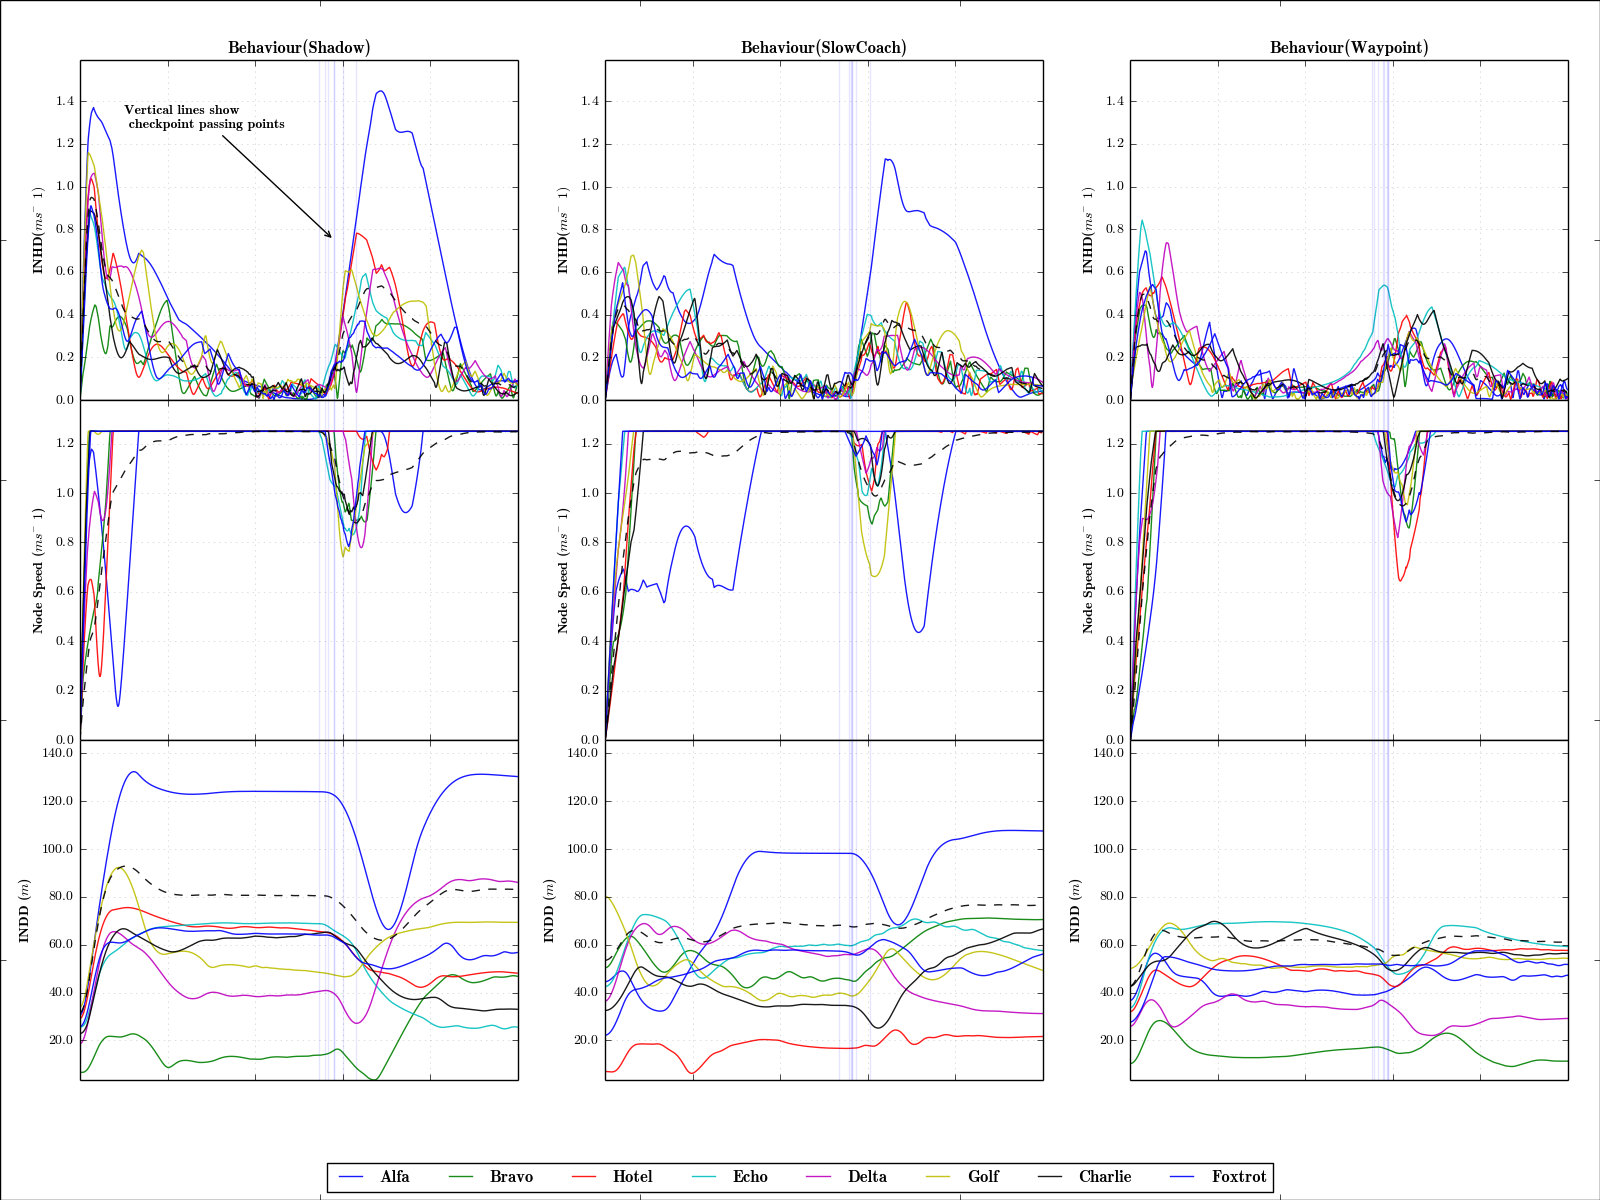
\includegraphics[height=0.8\paperheight]{img/BehaviourMetricComparison}
\end{center}
}
\frame{
\frametitle{Behavioural Trust Assessment in AUVs}
\begin{center}
  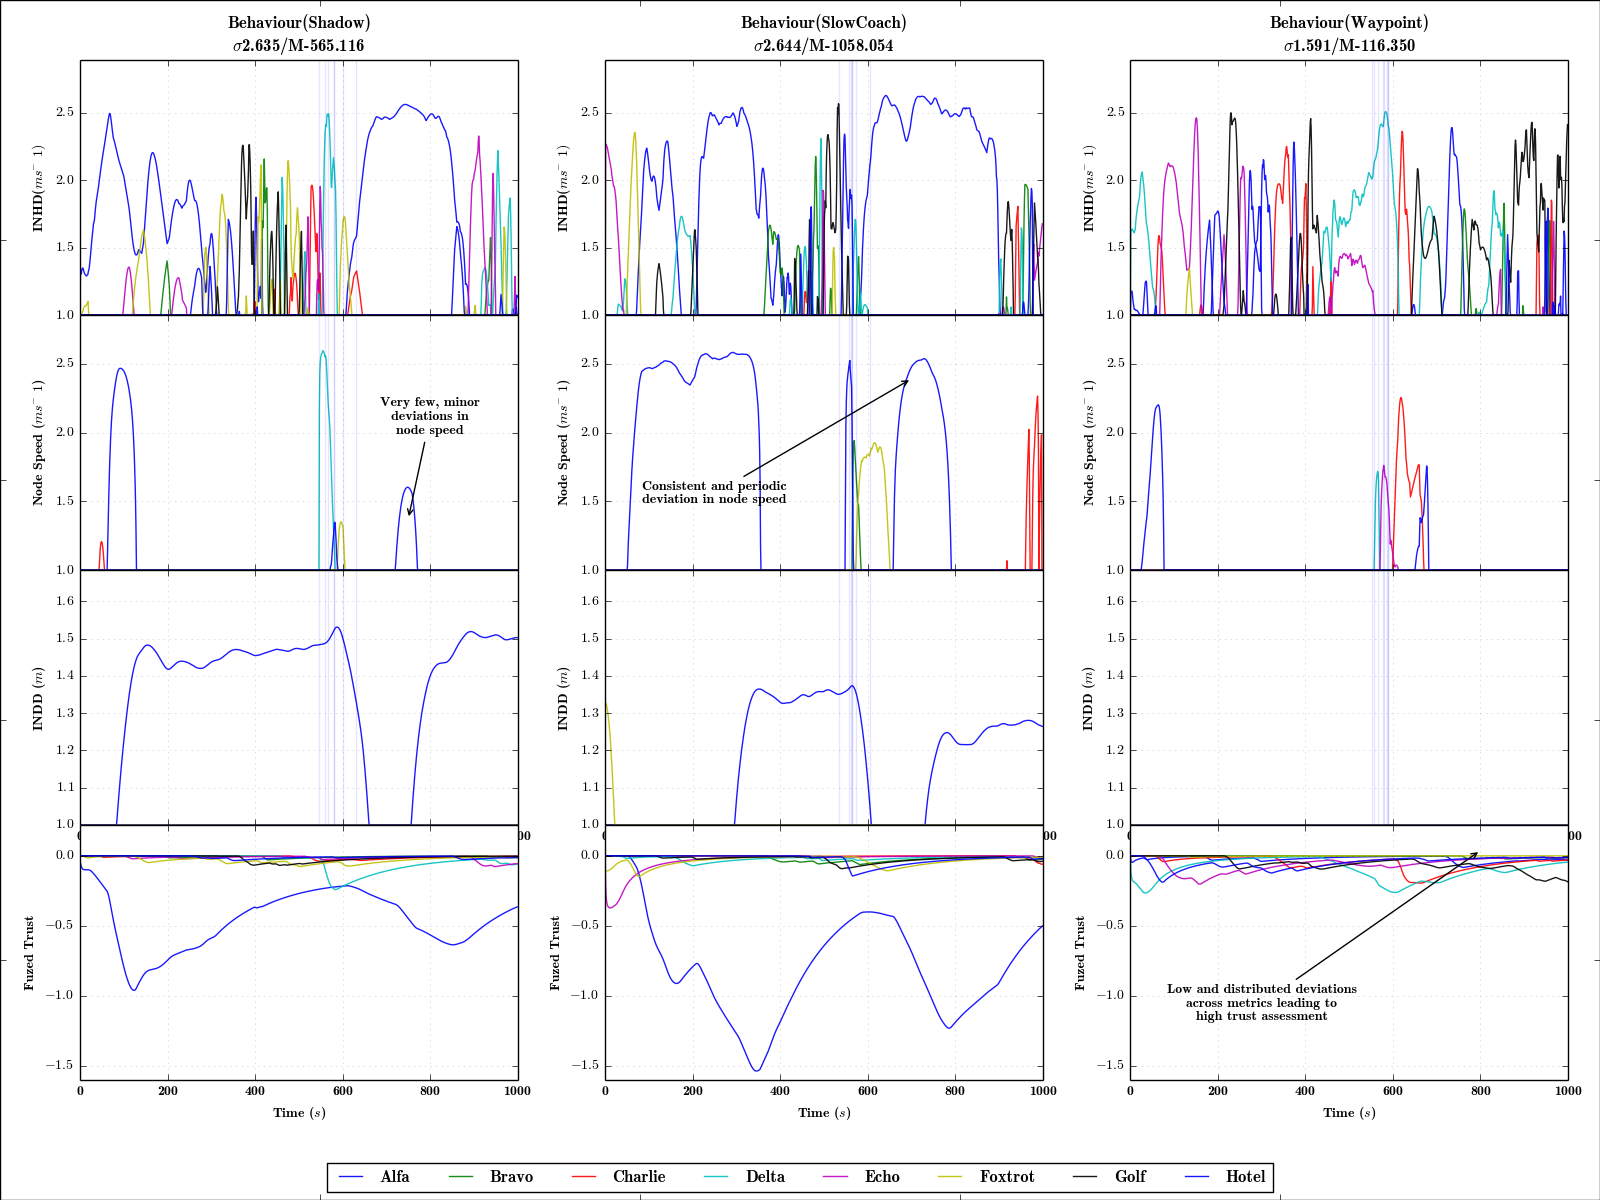
\includegraphics[height=0.8\paperheight]{img/BehaviourFusion}
\end{center}
}
\frame{
\frametitle{Behavioural Trust Assessment in AUVs}
\begin{itemize}
  \item Detection and identification based on basic weight-assessment classifier against windowed history of observations, with confidence based on a Grey Theoretic weight
  \item Currently >96\% statistical accuracy of detection and confidence, but this needs much more rigorous analysis
  \item Challenges to Trust assessment
  \begin{itemize}
    \item How to define optimality in trust assessment when dealing with multiple vectors and transitive trust?
    \item Is there a quantifiable benefit to cross-domain comparison beyond single vector Trust?
    \item Is there an optimal generic cross-domain comparator?
  \end{itemize}
\end{itemize}
}
\subsection{Publications}
\frame{
\frametitle{Current Publications}
\begin{itemize}
\item A Multi-Vector Trust Framework for Autonomous Systems \cite{Bolster2014}
  \begin{itemize}
  \item Symposium paper to the Association for the Advancement of Artificial Intelligence on the current state of work, presenting our progress towards multi-vector trust
  \end{itemize}


\item Analysis of Trust Interfaces in Autonomous and Semi-Autonomous Collaborative MHPC Operations \cite{Bolster2014a}
  \begin{itemize}
  \item Part of a Five-Eyes defence strategy programme (TTCP) for assuring C3I capabilities as part of FF2020
  \end{itemize}


\end{itemize}
}

\frame{
\frametitle{Development Plan}
\begin{enumerate}
  \item Behaviour Detection (Q3 14) - Formal Analysis of Behavioural Trust Systems
  \begin{itemize}
    \tiny
    \item INFOCOM 2015 (Aug 14)
    \item ASON 2014 : Seventh Int. WS on Autonomous Self-Organizing Networks (Aug 14)
    \item AHUC 2014 : The Fourth Int. WS on Ad Hoc and Ubiquitous Computing (Aug 14)
    \item ICCAR 2015 : WASET Int. Conf. on Control, Automation and Robotics (Dec 14)
  \end{itemize}
  \item MANET/Marine comparison (Q4 14) - Formal Comparison between Terrestrial MANET / Marine contexts
  \item Multi-Domain Trust Assessment (Q4 14) - Combination of Communicative and Physical Behaviour Trusts
  \begin{itemize}
    \tiny
    \item IEEE Trans. on Communications / Dependable and Secure Computing / Intelligent Systems
  \end{itemize}
  \item Reactionary/Perturbative Trust (Q1 15) - Exploration of reactionary behaviours for teams to 'shake down' suspects
  \begin{itemize}
    \tiny
    \item SASO15:Self-Adaptive and Self-Organizing Systems, 
    \item SEAMS15: Software Engineering for Adaptive and Self-Managing Systems
  \end{itemize}
\end{enumerate}
}


\section{Collaborations}
\frame{
\frametitle{Research Collaborations}
\begin{itemize}
  \item DSTL
    \begin{itemize}
      \item Visits and Placements (Summer  '13) at DSTL Porton Down and Portsdown West
      \item CDE Exhibition, London, (Spring '12)
      \item PhD National Conferences, Oxford and London (12/13)
      \item Direct Contribution to 5-Eyes programme on Autonomous Systems (13/14)
    \end{itemize}
  \item DGA/UPMC
    \begin{itemize}
      \item DGA Conference (Autumn, '12)
      \item Visits fo CRIIF (Autumn, '12)
    \end{itemize}
  \item NATO/CMRE
    \begin{itemize}
      \item UComms'12
      \item Visits \& Ongoing data sharing with CMRE(NURC) in La Spezzia
    \end{itemize}
  \item NPL/Plextek
    \begin{itemize}
      \item CDE Project on Precision Timing for Positioning with NPL/Plextek
      \item Simulation and Analysis of relevant drift characteristics; increasing positional accuracy by 40\%
    \end{itemize}
\end{itemize}
}


\section{Experience}
\frame{
\frametitle{Research Experience}
\begin{itemize}
  \item Project launched at QUB ECIT in 2011 under the DSTL/DGA Anglo French Defence Research Group PhD Programme 
  \item Primary Simulation/Analysis work done in 12/13
  \item Moved to UoL Oct 13 after 2 mth placement @ DSTL PDW Naval Systems / Information Systems departments.
\end{itemize}
\emph{Difficulties}
\begin{itemize}
  \item Move to UoL was challenging mid programme: new structures, requirements, etc. Incurred Delays
  \item Access to secure materials difficult (although placement helped a lot).
  \item Multiplicity of reporting (UoL, DSTL, Joint Programme, etc)
\end{itemize}

\emph{Benefits}
\begin{itemize}
  \item Flexibility in travel enabled international collaboration within and outside partners
  \item DSTL Placement extremely useful for context and background verification
\end{itemize}

}

%
\begin{frame}[t,allowframebreaks]
  \frametitle{References}
  \printbibliography[title=References]% [nottype=video]}
\end{frame}

\begin{frame}
  \centerline{The End}
\end{frame}
% End of slides
\end{document} 


